\chapter*{Appendices}
\markboth{Appendices}{}
\phantomsection
\addcontentsline{toc}{chapter}{Appendices}

\section*{Appendix A: Experimental Artifacts and Reproducibility Checklist}
\addcontentsline{toc}{section}{Appendix A: Experimental Artifacts and Reproducibility Checklist}

This appendix summarises the main artifacts used to reproduce the experiments described in chapters~4--6. The purpose is not to repeat the methodology chapter, but to provide a compact reference for the files, notebooks, result logs, and validation steps that were used during the local and \ac{HPC} stages of the work.

\subsection*{A.1 Project Artifact Map}
\addcontentsline{toc}{subsection}{A.1 Project Artifact Map}

\begin{table}[H]
\centering
\small
\begin{tabularx}{\textwidth}{>{\raggedright\arraybackslash}p{0.34\textwidth}>{\raggedright\arraybackslash}X}
\toprule
\textbf{Artifact} & \textbf{Role in the thesis workflow} \\
\midrule
\texttt{data/dummy\_data/} & Synthetic OrchestrAI enterprise corpus used by all experiments. The corpus contains 54 DOCX files grouped by department. \\
\texttt{notebooks/} & Local experiment notebooks using Ollama for generation and embeddings, and Milvus where vector-database retrieval is required. \\
\texttt{notebooks-hpc/} & \ac{HPC} experiment notebooks with the same six pipeline structures adapted for vLLM-based services. \\
\texttt{results\_logger.py} & Shared CSV logger that records the implementation name, scenario identifier, question, generated answer, retrieved sources, retrieved contexts, top-k values, and timing fields. \\
\texttt{ground\_truth\_builder.py} & Helper script for creating a manual ground-truth worksheet from generated results. \\
\texttt{deterministic\_eval.py} & Evaluation script that merges results with manual ground truth and computes answer-quality and retrieval-quality metrics. \\
\texttt{rag\_ground\_truth.csv} & Manual evaluation file containing reference answers, supporting documents, manual scores, labels, and notes. \\
\texttt{hpc\_results.csv} & \ac{HPC} timing output used for the local-versus-\ac{HPC} comparison. \\
\texttt{images/} & Figures and plots inserted into the thesis, including quality charts, timing charts, and speed-up visualisations. \\
\bottomrule
\end{tabularx}
\caption{Main artifacts used to reproduce and document the thesis experiments.}
\label{tab:appendix-artifact-map}
\end{table}

\subsection*{A.2 Pipeline Summary}
\addcontentsline{toc}{subsection}{A.2 Pipeline Summary}

\begin{table}[H]
\centering
\small
\begin{tabularx}{\textwidth}{>{\raggedright\arraybackslash}p{0.40\textwidth}>{\raggedright\arraybackslash}X}
\toprule
\textbf{Notebook} & \textbf{Purpose} \\
\midrule
\texttt{rag\_basic.ipynb} & In-memory dense retrieval baseline with no Milvus dependency. \\
\texttt{rag\_vectordb.ipynb} & Dense retrieval using Milvus as a persistent vector database. \\
\texttt{rag\_vectordb\_tuned.ipynb} & Milvus-backed dense retrieval with larger chunks and larger overlap. \\
\texttt{rag\_reranker.ipynb} & Milvus dense retrieval followed by cross-encoder reranking. \\
\texttt{rag\_hybrid.ipynb} & Milvus hybrid retrieval combining dense semantic search and sparse lexical matching. \\
\texttt{rag\_hybrid\_\&\_rerank.ipynb} & Hybrid retrieval followed by reranking before answer generation. \\
\bottomrule
\end{tabularx}
\caption{Implemented pipeline variants and their corresponding notebooks.}
\label{tab:appendix-pipeline-summary}
\end{table}

\subsection*{A.3 Scenario Set}
\addcontentsline{toc}{subsection}{A.3 Scenario Set}

\begin{table}[H]
\centering
\small
\begin{tabularx}{\textwidth}{>{\raggedright\arraybackslash}p{0.12\textwidth}>{\raggedright\arraybackslash}X>{\raggedright\arraybackslash}p{0.26\textwidth}}
\toprule
\textbf{Scenario} & \textbf{Question} & \textbf{Primary retrieval behaviour tested} \\
\midrule
1 & What is the first-response SLA for a Sev-1 support incident? & Single-document factual lookup. \\
2 & What steps must be completed before a new employee is considered ready for day one at OrchestrAI? & Checklist and procedure retrieval. \\
3 & A new engineer starts on Monday, but their laptop has not arrived and their required access is still pending. Which teams are involved and what should happen next? & Cross-team HR, IT, and access reasoning. \\
4 & Can OrchestrAI make an urgent hardware purchase without following the normal PO workflow if a warehouse outage is at risk? & Policy exception reasoning. \\
5 & A customer renewal is at risk because support cases are recurring, a requested feature is still unavailable, and replacement hardware is delayed. What should OrchestrAI do next, and which teams must be involved? & Multi-hop customer-risk analysis. \\
\bottomrule
\end{tabularx}
\caption{Scenario questions used across all six pipeline implementations.}
\label{tab:appendix-scenario-set}
\end{table}

\subsection*{A.4 Logged Fields}
\addcontentsline{toc}{subsection}{A.4 Logged Fields}

Each notebook writes rows using the shared logging schema below. This keeps local and \ac{HPC} outputs comparable at the workflow level.

\begin{itemize}
    \item \texttt{implementation}: pipeline identifier, such as \texttt{basic}, \texttt{vectordb}, or \texttt{hybrid\_rerank}.
    \item \texttt{scenario\_id}: scenario identifier used to distinguish the five questions per implementation.
    \item \texttt{question}: input question sent to the \ac{RAG} pipeline.
    \item \texttt{generated\_answer}: answer produced by the language model.
    \item \texttt{retrieved\_sources}: filenames of retrieved source documents.
    \item \texttt{retrieved\_departments}: department metadata associated with the retrieved documents.
    \item \texttt{retrieved\_contexts}: retrieved text fragments passed into the prompt.
    \item \texttt{num\_retrieved\_docs}: number of retrieved documents or chunks.
    \item \texttt{retriever\_top\_k} and \texttt{reranker\_top\_k}: retrieval and reranking limits used by the implementation.
    \item \texttt{indexing\_time\_s}, \texttt{retrieval\_time\_s}, and \texttt{generation\_time\_s}: application-level timing measurements in seconds.
\end{itemize}

\subsection*{A.5 Reproducibility Checklist}
\addcontentsline{toc}{subsection}{A.5 Reproducibility Checklist}

Before using a new run for analysis, the following checks should be completed:

\begin{enumerate}
    \item Confirm that the same 54 DOCX files are available under \texttt{data/dummy\_data/}.
    \item Confirm that Ollama, Milvus, or the \ac{HPC} vLLM services are running before executing notebooks that depend on them.
    \item Run the six notebooks in the documented order: basic, vector database, tuned vector database, reranker, hybrid, and hybrid with reranking.
    \item Verify that each implementation produces five result rows, one for each scenario.
    \item Verify that no result row has an empty generated answer, empty retrieved source list, or missing timing field.
    \item Build or update the manual ground-truth worksheet using evidence from the DOCX corpus only.
    \item Run the deterministic evaluation script after the manual scores, supporting documents, and reference answers have been completed.
    \item Copy only curated final results and figures into the final result directories used by the thesis.
\end{enumerate}

\newpage
\section*{Appendix B: Evaluation Rubric and Supporting Evidence Guide}
\addcontentsline{toc}{section}{Appendix B: Evaluation Rubric and Supporting Evidence Guide}

This appendix records the manual scoring logic used alongside the deterministic evaluation script. The manual assessment was necessary because automatic similarity metrics such as \ac{ROUGE-L}, \ac{BERTScore}, and sentence-embedding similarity can identify overlap with a reference answer, but they do not always determine whether an answer contains the operational detail required by the scenario.

\subsection*{B.1 Manual Answer Score}
\addcontentsline{toc}{subsection}{B.1 Manual Answer Score}

\begin{table}[H]
\centering
\small
\begin{tabularx}{\textwidth}{>{\raggedright\arraybackslash}p{0.18\textwidth}>{\raggedright\arraybackslash}p{0.24\textwidth}>{\raggedright\arraybackslash}X}
\toprule
\textbf{Score} & \textbf{Label} & \textbf{Interpretation} \\
\midrule
1.0 & \texttt{correct} & The answer is supported by the corpus and includes the required operational facts or steps for the scenario. Minor wording differences are acceptable. \\
0.5 & \texttt{partially\_correct} & The answer contains some relevant and supported information, but omits required details, mixes responsibilities, or does not fully answer the question. \\
0.0 & \texttt{incorrect} & The answer is unsupported, contradicts the corpus, retrieves the wrong operational process, or fails to answer the scenario. \\
\bottomrule
\end{tabularx}
\caption{Manual answer scoring rubric used in the thesis evaluation.}
\label{tab:appendix-manual-rubric}
\end{table}

\subsection*{B.2 Supporting Document Rules}
\addcontentsline{toc}{subsection}{B.2 Supporting Document Rules}

Supporting documents are recorded in \texttt{data/ground\_truth/rag\_ground\_truth.csv}. The following rules were used when filling the manual evidence fields:

\begin{itemize}
    \item Supporting documents must be selected from the DOCX corpus only.
    \item The \texttt{supporting\_documents} field should contain filenames that directly justify the reference answer.
    \item If a scenario requires more than one department, all essential supporting files should be recorded.
    \item Manual notes should explain omissions, unsupported statements, or incorrect operational reasoning.
    \item The score should be based on correctness against the corpus, not on whether the generated answer sounds fluent.
\end{itemize}

\subsection*{B.3 Deterministic Evaluation Outputs}
\addcontentsline{toc}{subsection}{B.3 Deterministic Evaluation Outputs}

After the manual worksheet is completed, the deterministic evaluation script produces per-row and per-implementation outputs. The key metrics are:

\begin{itemize}
    \item \textbf{Answer quality}: manual score, \ac{ROUGE-L} F1, \ac{BERTScore} F1, sentence-embedding semantic similarity, and answer length.
    \item \textbf{Retrieval quality}: retrieval hit, retrieval precision, retrieval recall, and retrieval F1.
    \item \textbf{Timing}: indexing time, retrieval time, and generation time averaged by implementation.
\end{itemize}

The local final outputs used in the thesis are stored in \texttt{data/results/final/}. The \ac{HPC} comparison uses timing rows generated by the \texttt{notebooks-hpc/} workflow. Since the \ac{HPC} phase was used for timing comparison only, the main answer-quality and retrieval-quality interpretation is based on the local evaluation workflow.

\newpage
\section*{Appendix C: Supplementary Figures}
\addcontentsline{toc}{section}{Appendix C: Supplementary Figures}

This appendix includes supplementary figures generated during the project. They support the implementation and timing discussion but are kept outside the main chapters so that the core results chapter remains focused on the most important comparisons.


\begin{figure}[H]
    \centering
    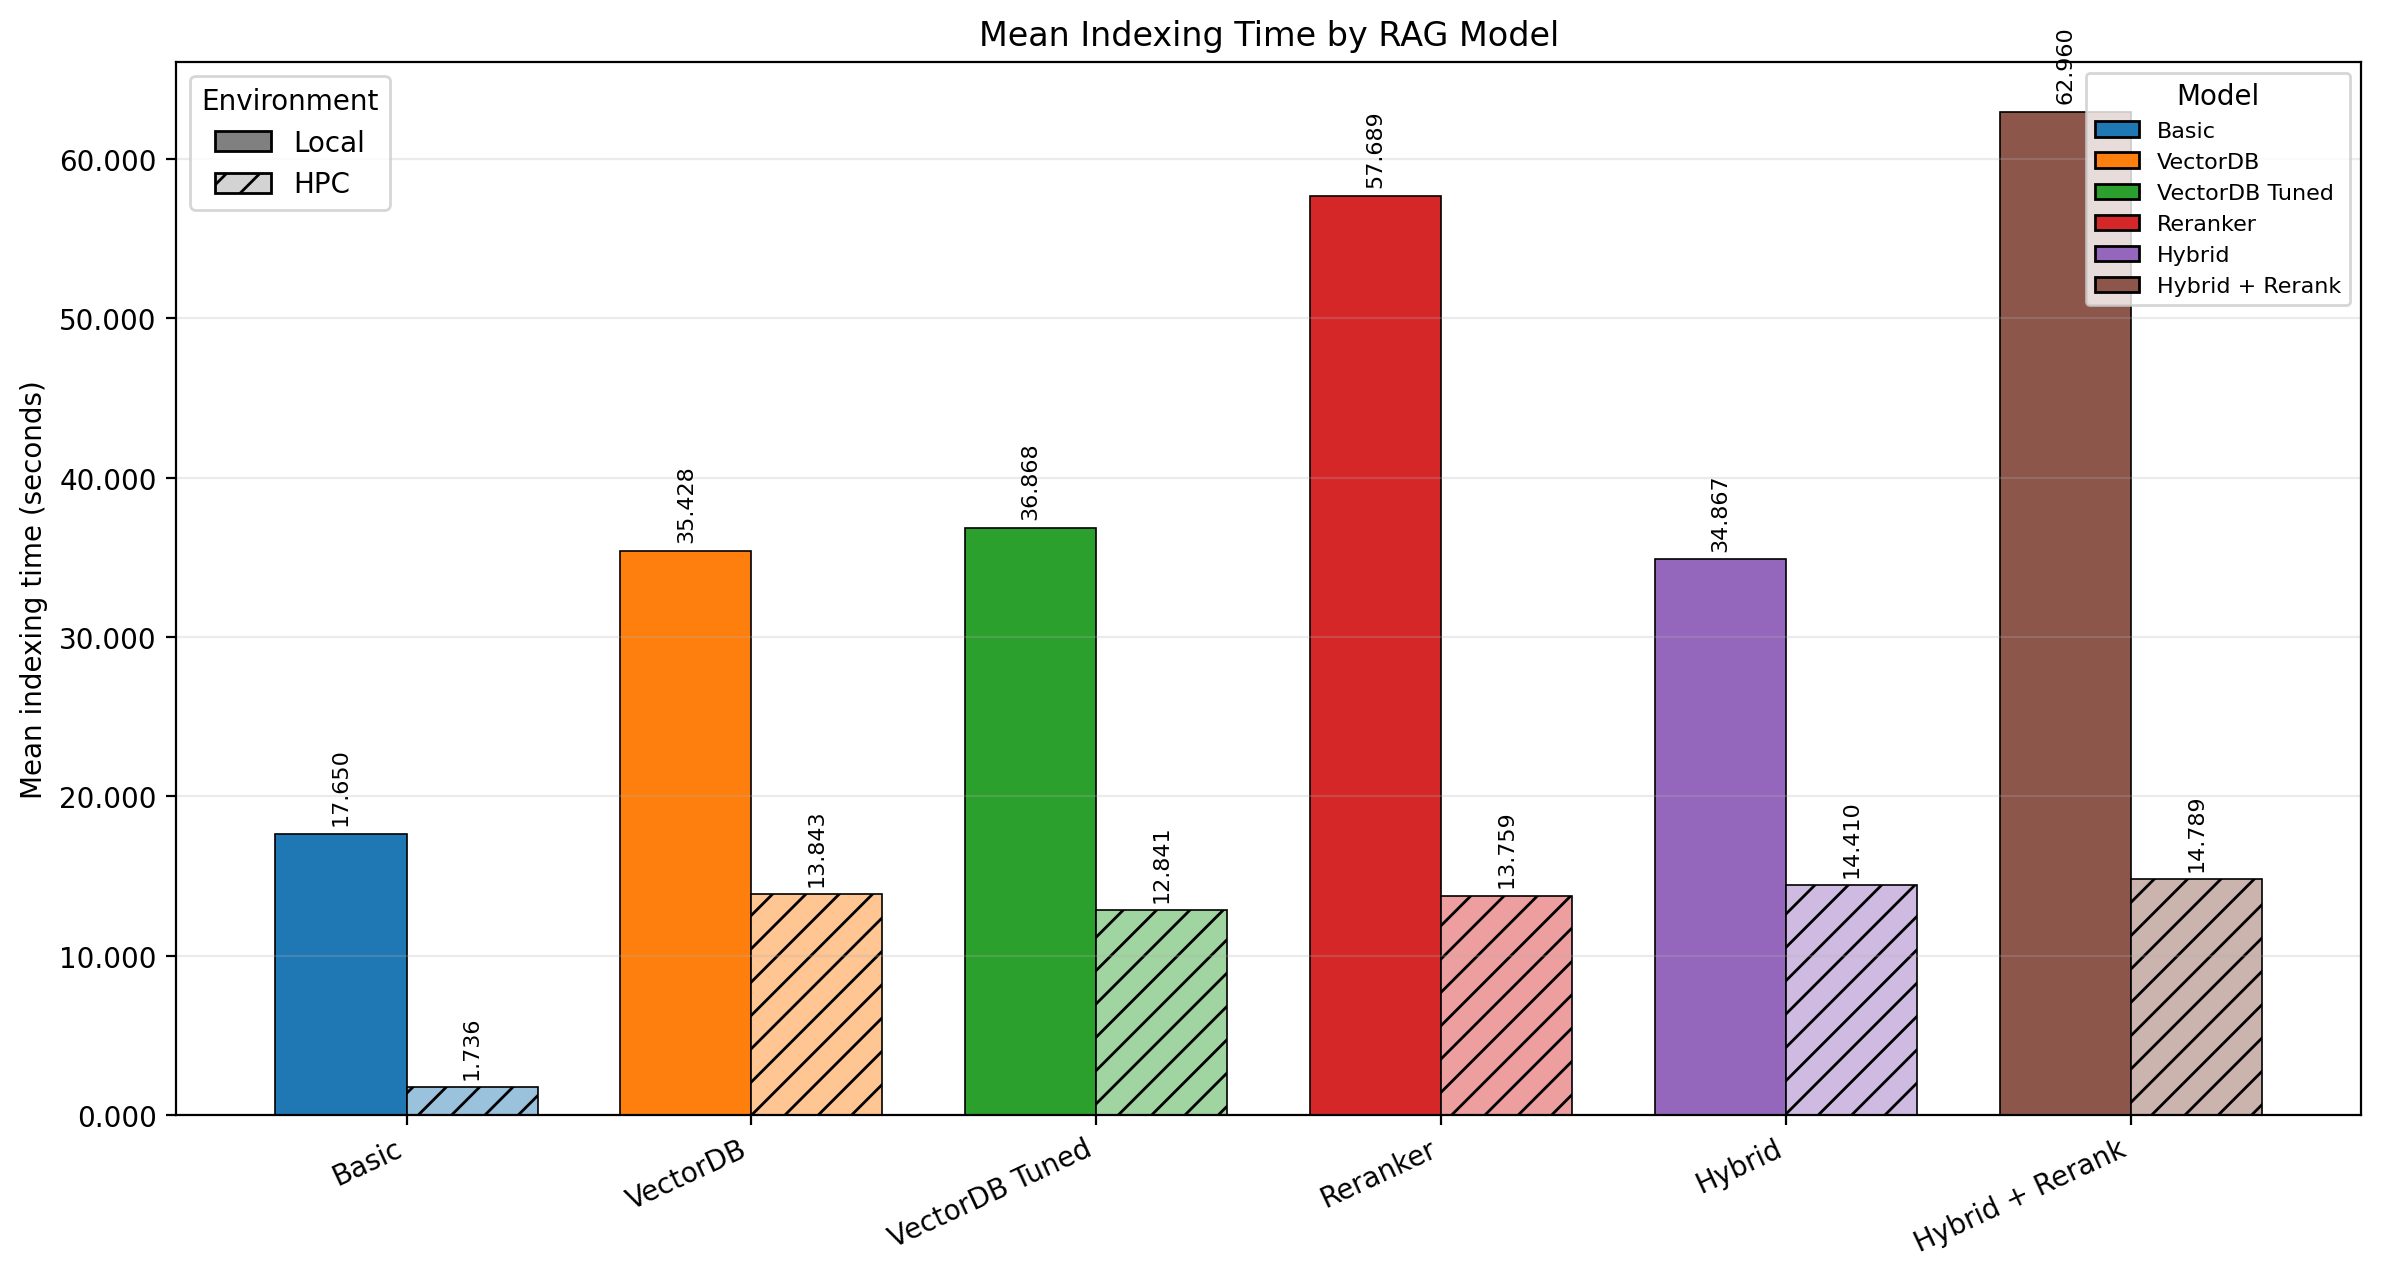
\includegraphics[width=\textwidth]{images/mean_indexing_time.png}
    \caption{Mean indexing time by pipeline and execution environment.}
    \label{fig:appendix-mean-indexing-time}
\end{figure}

\begin{figure}[H]
    \centering
    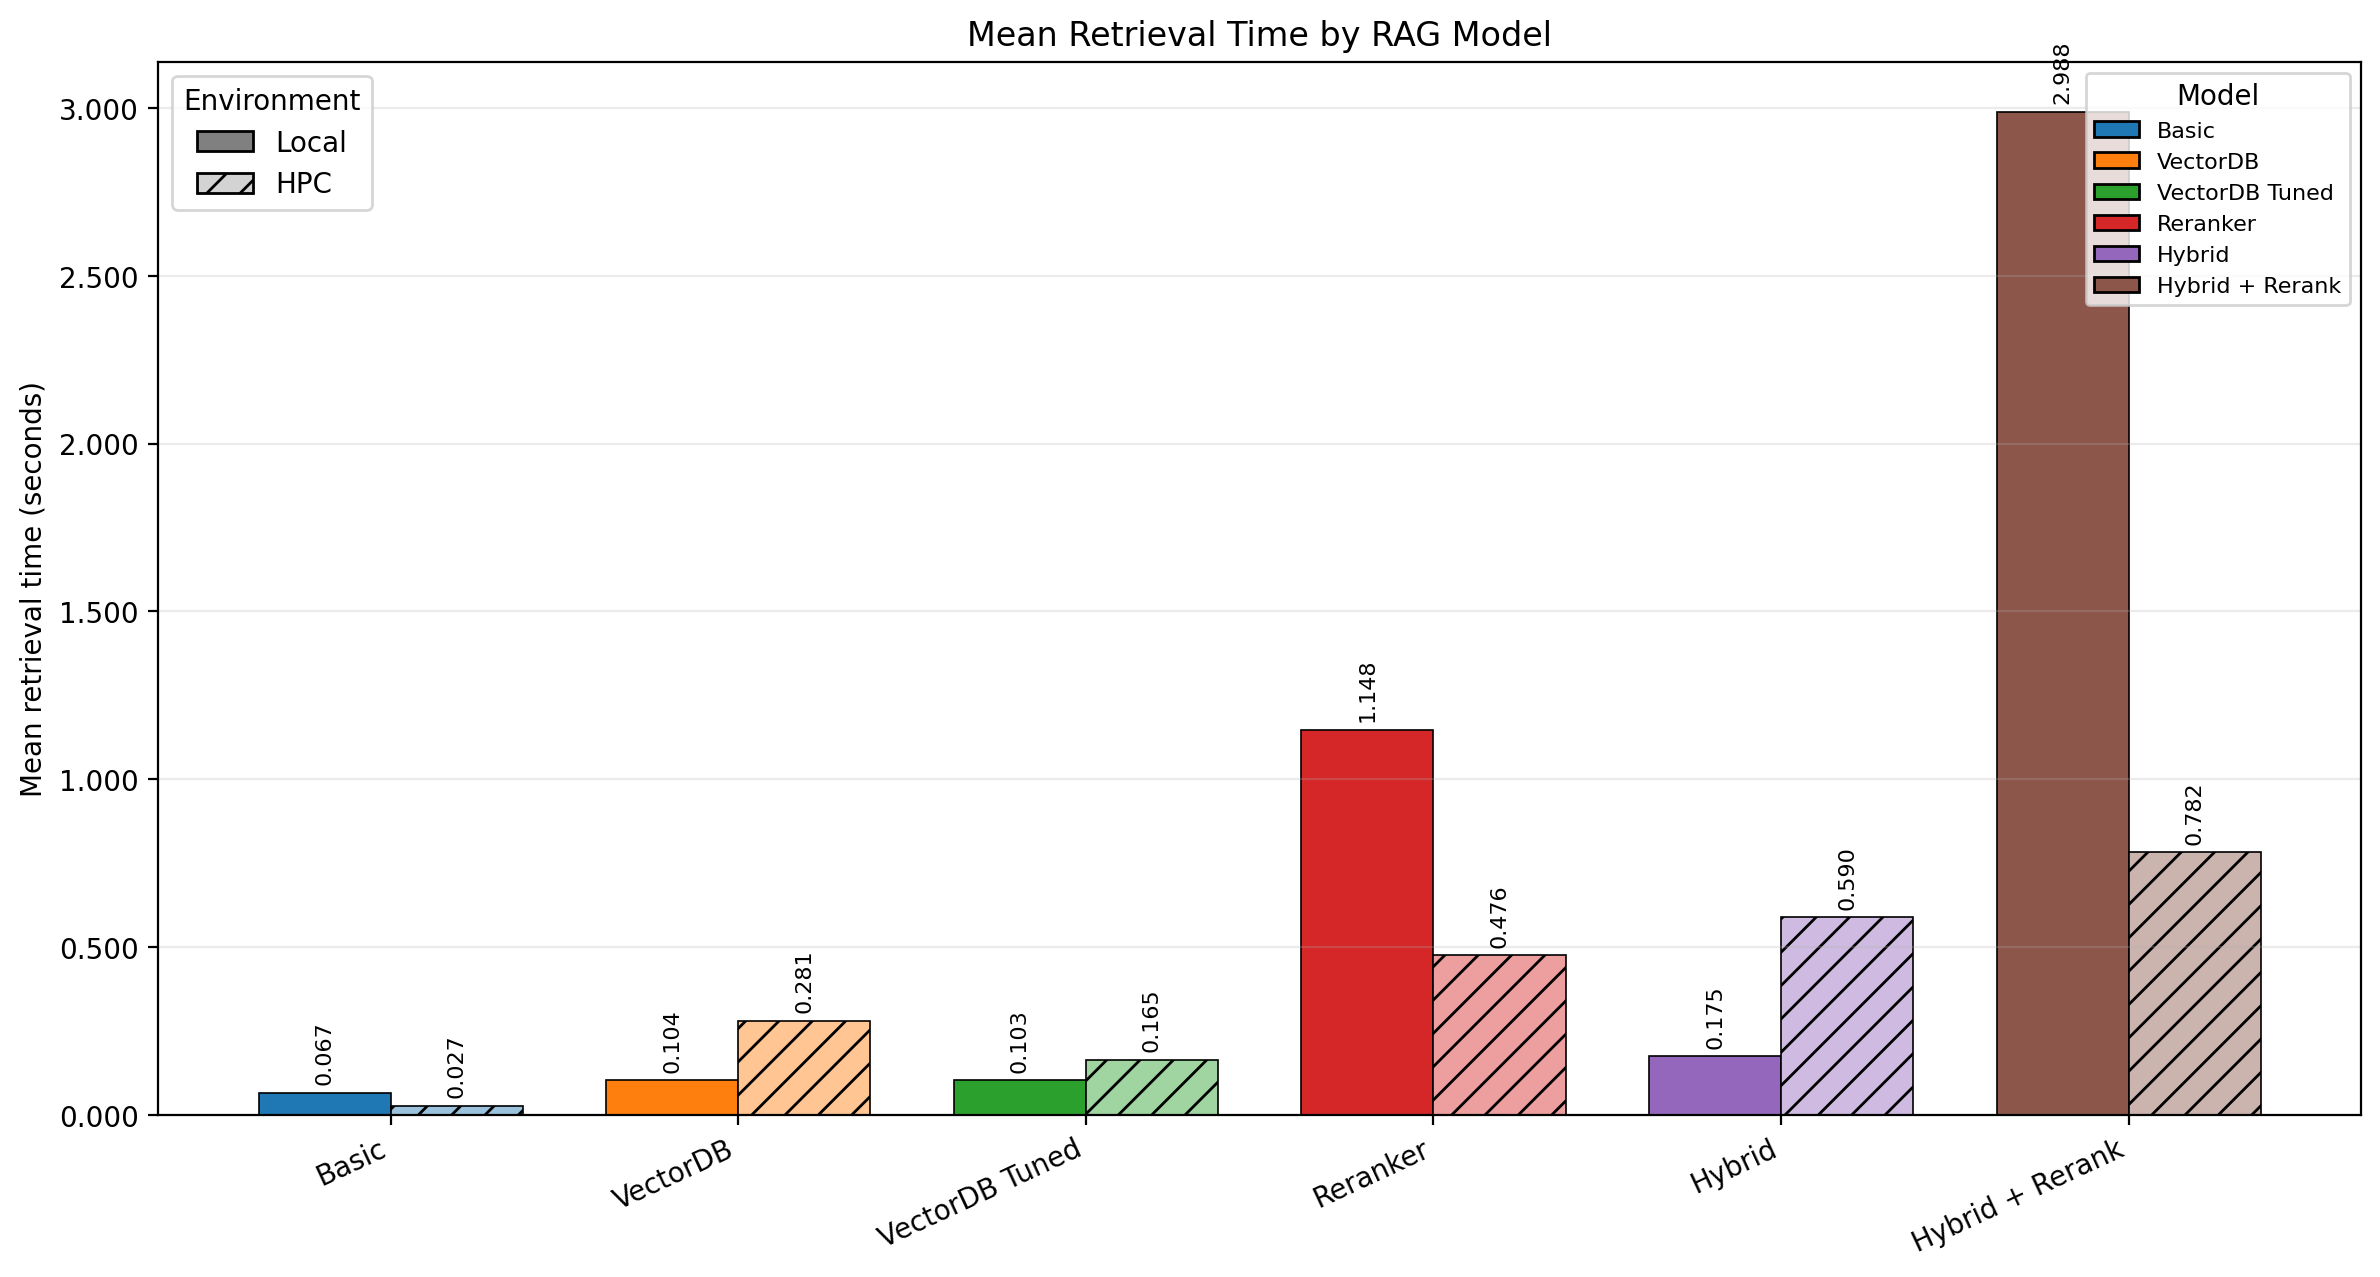
\includegraphics[width=\textwidth]{images/mean_retrieval_time.png}
    \caption{Mean retrieval time by pipeline and execution environment.}
    \label{fig:appendix-mean-retrieval-time}
\end{figure}

\begin{figure}[H]
    \centering
    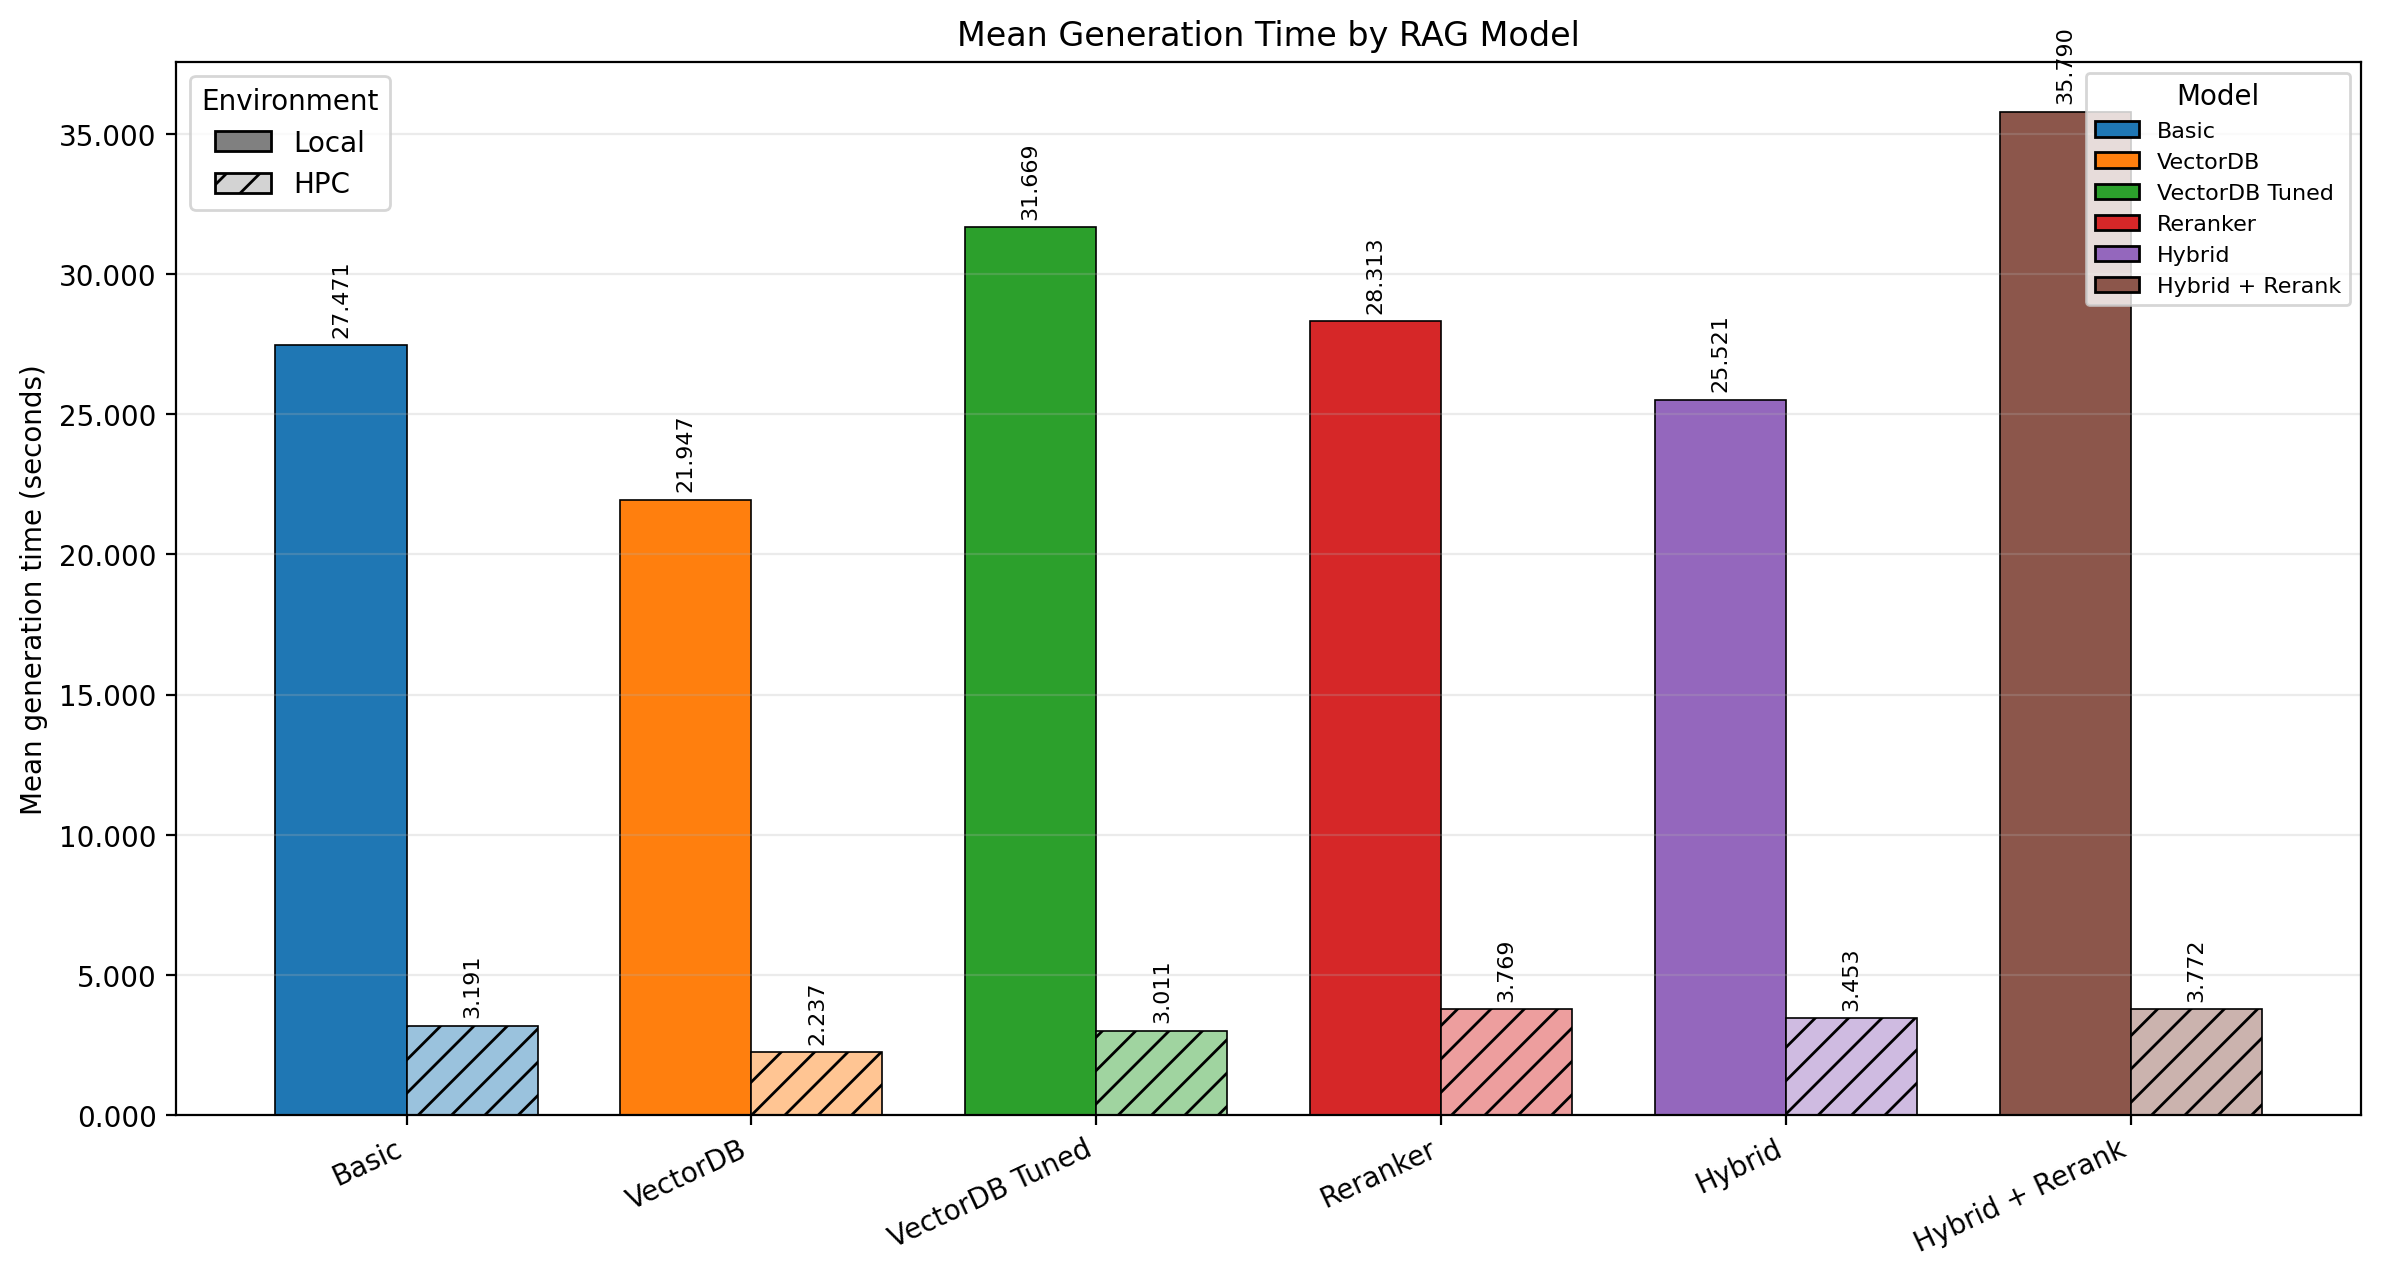
\includegraphics[width=\textwidth]{images/mean_generation_time.png}
    \caption{Mean generation time by pipeline and execution environment.}
    \label{fig:appendix-mean-generation-time}
\end{figure}

\begin{figure}[H]
    \centering
    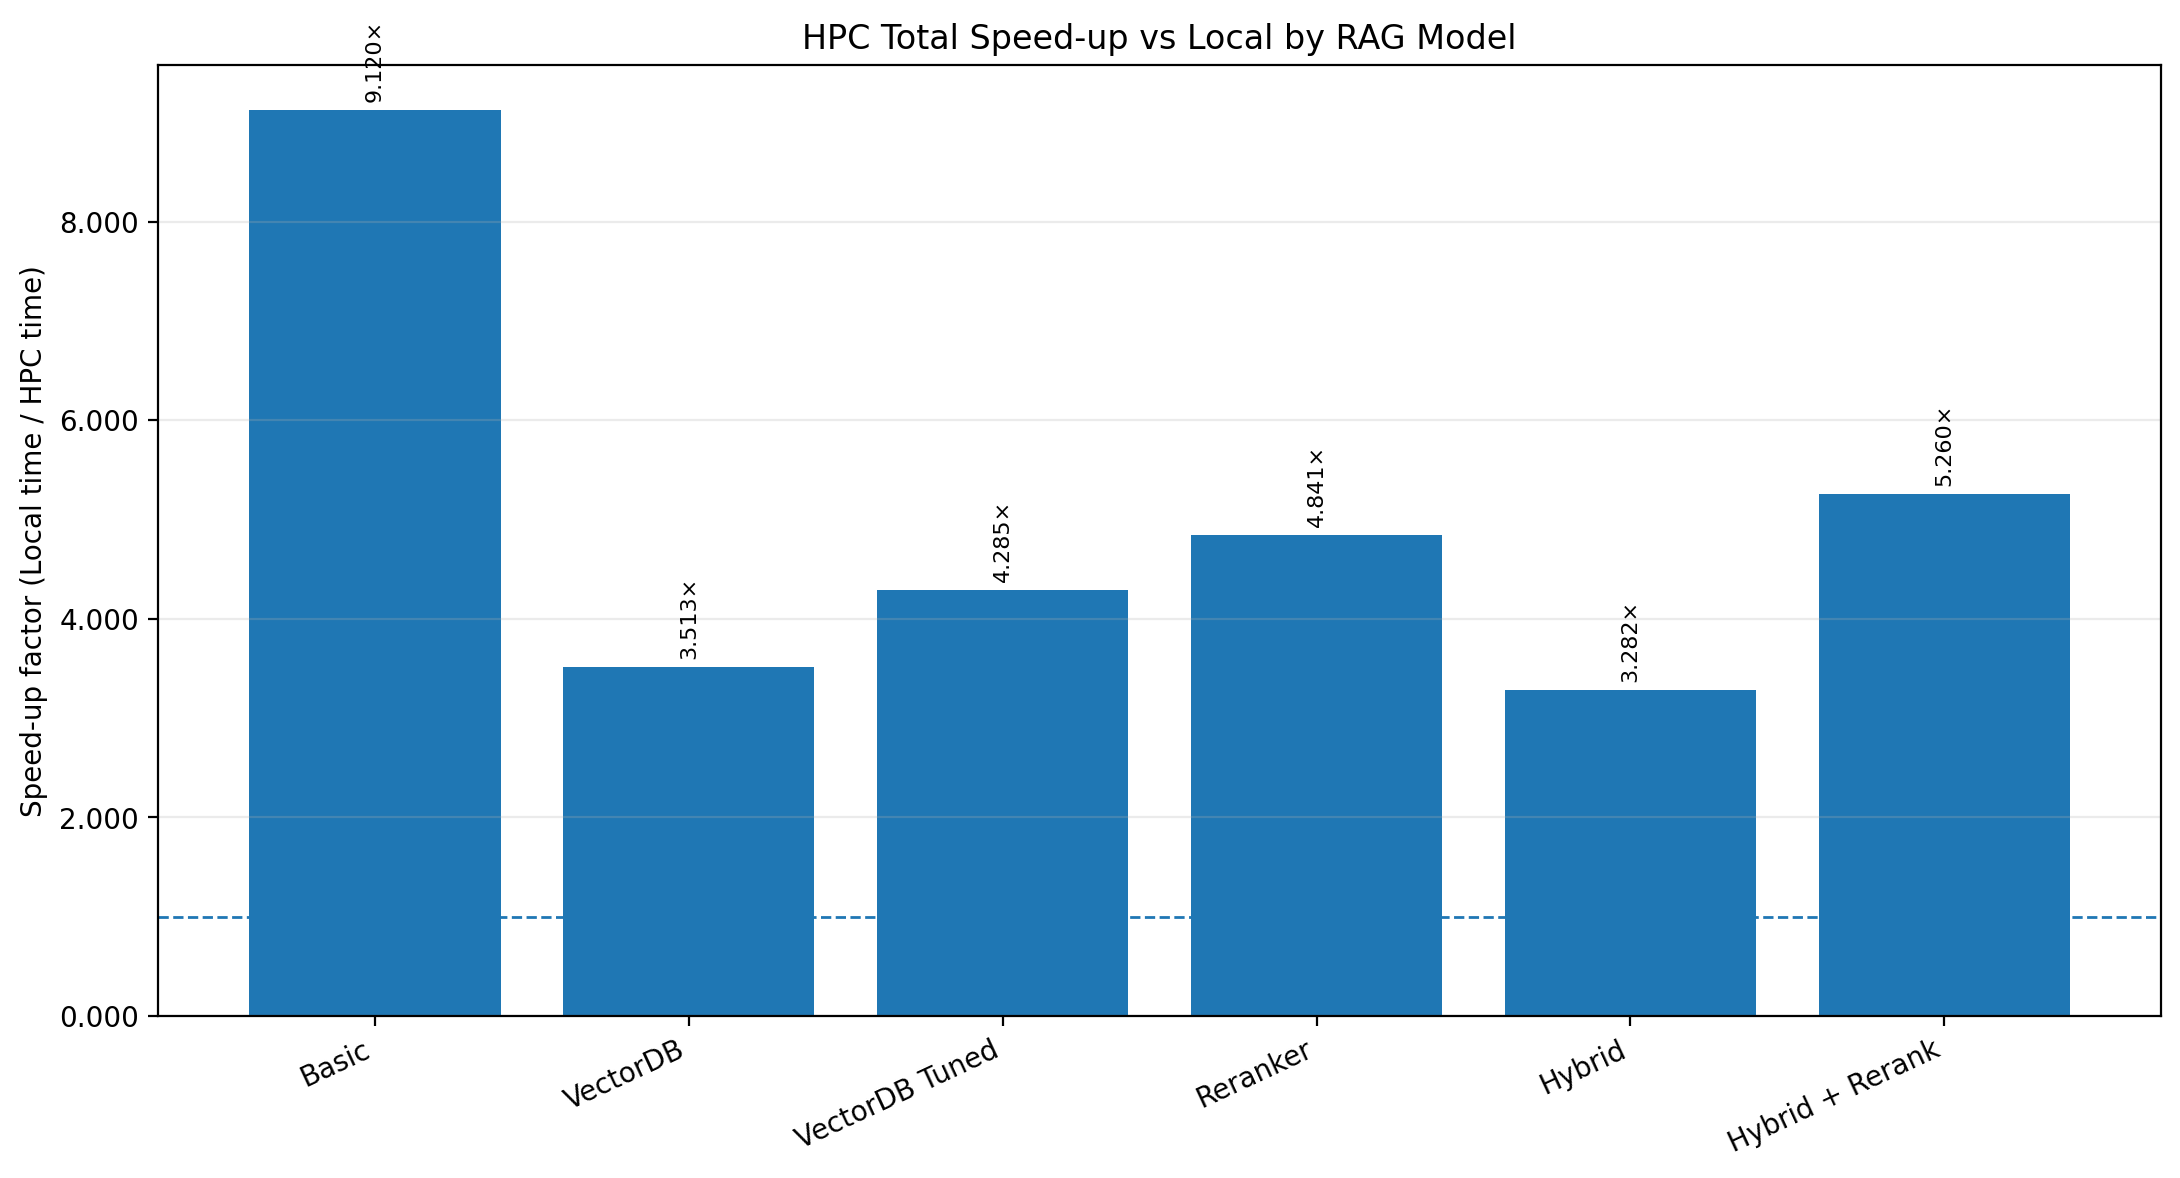
\includegraphics[width=\textwidth]{images/total_speedup_factor.png}
    \caption{Total speed-up factor for each RAG pipeline when comparing local and HPC execution.}
    \label{fig:appendix-total-speedup-factor}
\end{figure}